\section{Introduction}\label{sec:intro}

\begin{itemize}
    \item The importance of relational learning; lots of references.
    \item We propose a framework analogous to CNNs, but for relational learning
    \item Advantages: modularity, compositionality, hierarchical.
    \item Experiments showing advantages over existing frameworks. 
    \item Main contribution: Framework for relational learning that shares the strengths of CNNs for relational learning
\end{itemize}

Modeling of relations between objects is important to a range of machine learning problems:
Image analysis might rely on comparing objects in terms of relations that extract color, 
size, or texture features; natural language analysis may use relations that are based on syntactic or semantic features of pairs of words. While some machine learning tasks are ``purely relational'' and rely exclusively on identification and processing of relational information, others combine extraction of relations with function approximation. 

Given the key role that the processing of relations has in machine learning, it is important to explore learning architectures that support processing of relations in a natural, expressive, and efficient manner. In this paper we propose a framework we call ``relational convolution networks'' that provide for relational learning what standard convolutional neural networks provide for typical image processing applications. A schematic of the proposed architecture is shown in Figure~\ref{fig:relconv_architecture},
which supports hierarchical relational machine learning. At each layer, the multi-head relation module takes a sequence of objects as input and produces a relation tensor representing the relations between each pair of objects. The relational convolution layer then transforms the relation tensor into a sequence of objects, each describing the relations within some group of objects at the previous layer. The next layer receives this sequence of objects as input and again models the relations within it. Thus, each layer computes relational features of a higher-order (i.e., relations on relations). This is analogous to the manner that convolutional layers in a CNN can be composed to construct a chain of feature maps. 


% \begin{figure}[!ht]
%     \centering
%     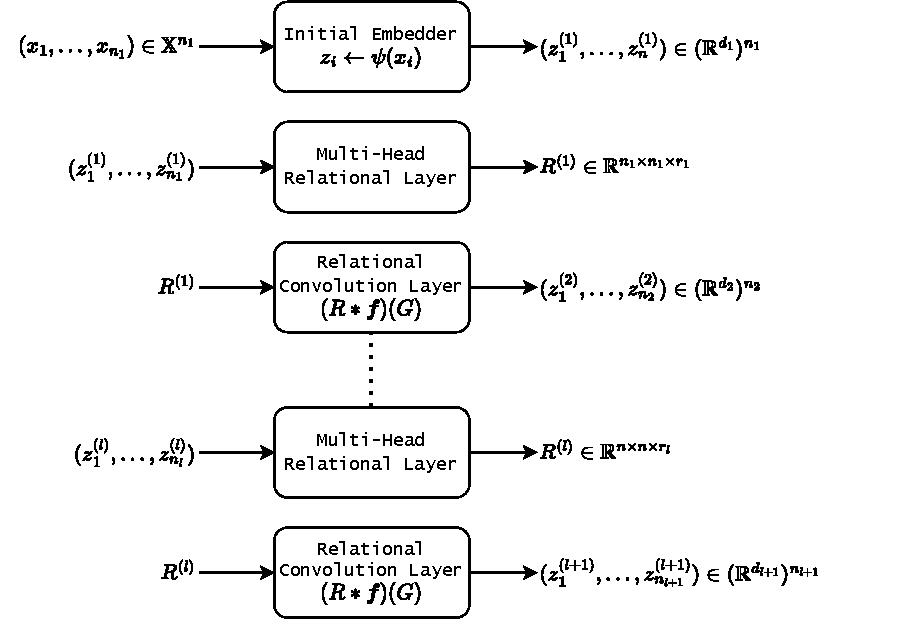
\includegraphics[width=0.75\textwidth]{figs/relational_framework.pdf}
%     \caption{A depiction of our proposed framework for hierarchical relational machine learning. At each layer, the multi-head relation module takes a sequence of objects as input and produces a relation tensor representing the relations between each pair of objects. The relational convolution layer then transforms the relation tensor into a sequence of objects each describing the relations within some group of objects at the previous layer. The next layer receives this sequence of objects as input and again models the relations within it. Thus, each layer computes relational features of a higher-order (i.e., relations on relations). \textit{Legend}: $d_l$ represents the dimension of the objects at layer $l$; $z_i^{(l)}$ is the $i$th object at the $l$th layer; $R^{(k)}$ is the relation tensor at layer $l$; $r_l$ is the dimension of the relations at layer $l$; $n_l$ is the number of objects at layer $l$.}\label{fig:relational_framework}
% \end{figure}


\begin{figure}[!ht]
    \centering
    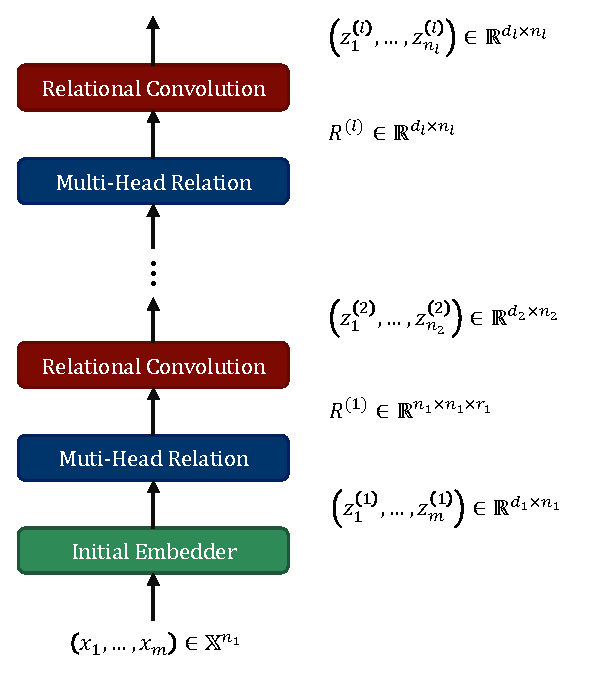
\includegraphics{figs/relconv_architecture.pdf}
    \caption{}\label{fig:relconv_architecture}
\end{figure}